% 2-15-rb-tree.tex

%%%%%%%%%%%%%%%%%%%%
\documentclass[a4paper, justified]{tufte-handout}

% hw-preamble.tex

% geometry for A4 paper
% See https://tex.stackexchange.com/a/119912/23098
\geometry{
  left=20.0mm,
  top=20.0mm,
  bottom=20.0mm,
  textwidth=130mm, % main text block
  marginparsep=5.0mm, % gutter between main text block and margin notes
  marginparwidth=50.0mm % width of margin notes
}

% for colors
\usepackage{xcolor} % usage: \color{red}{text}
% predefined colors
\newcommand{\red}[1]{\textcolor{red}{#1}} % usage: \red{text}
\newcommand{\blue}[1]{\textcolor{blue}{#1}}
\newcommand{\teal}[1]{\textcolor{teal}{#1}}

\usepackage{todonotes}

% heading
\usepackage{sectsty}
\setcounter{secnumdepth}{2}
\allsectionsfont{\centering\huge\rmfamily}

% for Chinese
\usepackage{xeCJK}
\usepackage{zhnumber}
\setCJKmainfont[BoldFont=FandolSong-Bold.otf]{FandolSong-Regular.otf}

% for fonts
\usepackage{fontspec}
\newcommand{\song}{\CJKfamily{song}} 
\newcommand{\kai}{\CJKfamily{kai}} 

% To fix the ``MakeTextLowerCase'' bug:
% See https://github.com/Tufte-LaTeX/tufte-latex/issues/64#issuecomment-78572017
% Set up the spacing using fontspec features
\renewcommand\allcapsspacing[1]{{\addfontfeature{LetterSpace=15}#1}}
\renewcommand\smallcapsspacing[1]{{\addfontfeature{LetterSpace=10}#1}}

% for url
\usepackage{hyperref}
\hypersetup{colorlinks = true, 
  linkcolor = teal,
  urlcolor  = teal,
  citecolor = blue,
  anchorcolor = blue}

\newcommand{\me}[4]{
    \author{
      {\bfseries 姓名:}\underline{#1}\hspace{2em}
      {\bfseries 学号:}\underline{#2}\hspace{2em}\\[10pt]
      {\bfseries 评分:}\underline{#3\hspace{3em}}\hspace{2em}
      {\bfseries 评阅:}\underline{#4\hspace{3em}}
  }
}

% Please ALWAYS Keep This.
\newcommand{\noplagiarism}{
  \begin{center}
    \fbox{\begin{tabular}{@{}c@{}}
      请独立完成作业,不得抄袭。\\
      若得到他人帮助, 请致谢。\\
      若参考了其它资料,请给出引用。\\
      鼓励讨论,但需独立书写解题过程。
    \end{tabular}}
  \end{center}
}

\newcommand{\goal}[1]{
  \begin{center}{\fcolorbox{blue}{yellow!60}{\parbox{0.50\textwidth}{\large 
    \begin{itemize}
      \item 体会``思维的乐趣''
      \item 初步了解递归与数学归纳法 
      \item 初步接触算法概念与问题下界概念
    \end{itemize}}}}
  \end{center}
}

% Each hw consists of four parts:
\newcommand{\beginrequired}{\hspace{5em}\section{作业 (必做部分)}}
\newcommand{\beginoptional}{\section{作业 (选做部分)}}
\newcommand{\beginot}{\section{Open Topics}}
\newcommand{\begincorrection}{\section{订正}}
\newcommand{\beginfb}{\section{反馈}}

% for math
\usepackage{amsmath, mathtools, amsfonts, amssymb}
\newcommand{\set}[1]{\{#1\}}

% define theorem-like environments
\usepackage[amsmath, thmmarks]{ntheorem}

\theoremstyle{break}
\theorempreskip{2.0\topsep}
\theorembodyfont{\song}
\theoremseparator{}
\newtheorem{problem}{题目}[subsection]
\renewcommand{\theproblem}{\arabic{problem}}
\newtheorem{ot}{Open Topics}

\theorempreskip{3.0\topsep}
\theoremheaderfont{\kai\bfseries}
\theoremseparator{:}
\theorempostwork{\bigskip\hrule}
\newtheorem*{solution}{解答}
\theorempostwork{\bigskip\hrule}
\newtheorem*{revision}{订正}

\theoremstyle{plain}
\newtheorem*{cause}{错因分析}
\newtheorem*{remark}{注}

\theoremstyle{break}
\theorempostwork{\bigskip\hrule}
\theoremsymbol{\ensuremath{\Box}}
\newtheorem*{proof}{证明}

% \newcommand{\ot}{\blue{\bf [OT]}}

% for figs
\renewcommand\figurename{图}
\renewcommand\tablename{表}

% for fig without caption: #1: width/size; #2: fig file
\newcommand{\fig}[2]{
  \begin{figure}[htbp]
    \centering
    \includegraphics[#1]{#2}
  \end{figure}
}
% for fig with caption: #1: width/size; #2: fig file; #3: caption
\newcommand{\figcap}[3]{
  \begin{figure}[htbp]
    \centering
    \includegraphics[#1]{#2}
    \caption{#3}
  \end{figure}
}
% for fig with both caption and label: #1: width/size; #2: fig file; #3: caption; #4: label
\newcommand{\figcaplbl}[4]{
  \begin{figure}[htbp]
    \centering
    \includegraphics[#1]{#2}
    \caption{#3}
    \label{#4}
  \end{figure}
}
% for margin fig without caption: #1: width/size; #2: fig file
\newcommand{\mfig}[2]{
  \begin{marginfigure}
    \centering
    \includegraphics[#1]{#2}
  \end{marginfigure}
}
% for margin fig with caption: #1: width/size; #2: fig file; #3: caption
\newcommand{\mfigcap}[3]{
  \begin{marginfigure}
    \centering
    \includegraphics[#1]{#2}
    \caption{#3}
  \end{marginfigure}
}

\usepackage{fancyvrb}

% for algorithms
\usepackage[]{algorithm}
\usepackage[]{algpseudocode} % noend
% See [Adjust the indentation whithin the algorithmicx-package when a line is broken](https://tex.stackexchange.com/a/68540/23098)
\newcommand{\algparbox}[1]{\parbox[t]{\dimexpr\linewidth-\algorithmicindent}{#1\strut}}
\newcommand{\hStatex}[0]{\vspace{5pt}}
\makeatletter
\newlength{\trianglerightwidth}
\settowidth{\trianglerightwidth}{$\triangleright$~}
\algnewcommand{\LineComment}[1]{\Statex \hskip\ALG@thistlm \(\triangleright\) #1}
\algnewcommand{\LineCommentCont}[1]{\Statex \hskip\ALG@thistlm%
  \parbox[t]{\dimexpr\linewidth-\ALG@thistlm}{\hangindent=\trianglerightwidth \hangafter=1 \strut$\triangleright$ #1\strut}}
\makeatother

% for footnote/marginnote
% see https://tex.stackexchange.com/a/133265/23098
\usepackage{tikz}
\newcommand{\circled}[1]{%
  \tikz[baseline=(char.base)]
  \node [draw, circle, inner sep = 0.5pt, font = \tiny, minimum size = 8pt] (char) {#1};
}
\renewcommand\thefootnote{\protect\circled{\arabic{footnote}}} % feel free to modify this file
%%%%%%%%%%%%%%%%%%%%
\title{第3-7讲: 图的遍历}
\me{朱宇博}{191220186}{}{}
\date{\zhtoday} % or like 2019年9月13日
%%%%%%%%%%%%%%%%%%%%
\begin{document}
\maketitle
%%%%%%%%%%%%%%%%%%%%
\noplagiarism % always keep this line
%%%%%%%%%%%%%%%%%%%%
\begin{abstract}
  % \begin{center}{\fcolorbox{blue}{yellow!60}{\parbox{0.65\textwidth}{\large 
  %   \begin{itemize}
  %     \item 
  %   \end{itemize}}}}
  % \end{center}
\end{abstract}
%%%%%%%%%%%%%%%%%%%%
\beginrequired

%%%%%%%%%%%%%%%
\begin{problem}[TC 22.1-3]
The \textbf{transpose} of a directed graph $G=(V,E)$ is the graph $G^T=(V,E^T)$, where $E^T=\{(v,u)\in V\times V:(u,v) \in E\}$.Thus,$G^T$ is $G$ with all its edge sreversed. Describe efficient algorithms for computing $G^T$ from $G$, for both the adjacency-list and adjacency-matrix representations of $G$. Analyze the running times of your algorithms.
\end{problem}

\begin{solution}
\noindent
\begin{algorithm}
\caption{adjacency-list}\label{euclid}
\begin{algorithmic}[1]
\Procedure{adjacency-list }{V}
\For {$x \in V$}
	\For{$y \in E(x)$}
	 	\State add $x$ to $E^{1}(y)$
        \EndFor
\EndFor
\EndProcedure
\end{algorithmic}
\end{algorithm}
\noindent
\noindent
\begin{algorithm}
\caption{adjacency-matrix}\label{euclid}
\begin{algorithmic}[1]
\Procedure{adjacency-matrix }{V}
\For {$x \in V$}
	\For{$y \in V$}
	 	\If {$(x,y) \in E$}
			\State add $(y,x)$ to $E^{1}$
		\EndIf
        \EndFor
\EndFor
\EndProcedure
\end{algorithmic}
\end{algorithm}
\noindent
对于邻接表,每个点、每条边被遍历常数次,时间复杂度$O(V+E)$\\
对于邻接矩阵,两重循环,每层$O(V)$,时间复杂度$O(V^2)$
\end{solution}
%%%%%%%%%%%%%%%

%%%%%%%%%%%%%%%
\begin{problem}[TC 22.1-8]
Suppose that instead of a linked list, each array entry $Adj[u]$ is a hash table containing the vertices 􏰁 for which $(u,v)\in E$. If all edge lookups are equally likely, what is the expected time to determine whether an edge is in the graph? What disadvantages does this scheme have? Suggest an alternate data structure for each edge list that solves these problems. Does your alternative have disadvantages compared to the hash table?
\end{problem}

\begin{solution}
在散列表中,单次询问的期望复杂度为$O(1)$\\
缺点: 其最坏情况下,复杂度可以达到$O(n)$\\
可以用$set$结合维护相连边的集合\\
缺点:期望复杂度为$O(\lg n)$,不如哈希表
\end{solution}
%%%%%%%%%%%%%%%

%%%%%%%%%%%%%%%
\begin{problem}[TC 22.2-3("lines 5 and 14" 改为"line 18")]
Show that using a single bit to store each vertex color suffices by arguing that the BFS procedure would produce the same result if lines 18 were removed.
\end{problem}

\begin{solution}
删除$18$行之后,点的颜色只有灰色和白色。在这种情况下,未遍历到的点都为白色,遍历到的点全为灰色。\\
由算法可知每次访问新节点,必为白色。而在访问之后,会将其赋值成黑色。\\
每个节点仍只被遍历一次,bfs算法和原算法等价。
\end{solution}
%%%%%%%%%%%%%%%

%%%%%%%%%%%%%%%
\begin{problem}[TC 22.2-4]
What is the running time of BFS if we represent its input graph by an adjacency matrix and modify the algorithm to handle this form of input?
\end{problem}

\begin{solution}
复杂度为$O(V^2)$。$bfs$算法中,能访问到的每个点,仅会访问一次,且在该点扫描连边时,会遍历所有的点。
\end{solution}
%%%%%%%%%%%%%%%

%%%%%%%%%%%%%%%
\begin{problem}[TC 22.2-5]
Argue that in a breadth-first search, the value $u,d$ assigned to a vertex $u$ is independent of the order in which the vertices appear in each adjacency list. Using Figure 22.3 as an example, show that the breadth-first tree computed by BFS can depend on the ordering within adjacency lists.
\end{problem}

\begin{solution}
(1)\\
在$bfs$算法中,对于每一顶点$u$,除了他在$bfs$中已经被染色的点外,其余节点$v$都满足$d[v] = d[u] + 1$,和其在邻接表中顺序无关。对于已经被染色的点,也仅仅和其到源点$s$的距离相关,和其在邻接表中顺序无关。\\
\newpage
(2)\\
 \begin{figure}[htbp]
    \centering
    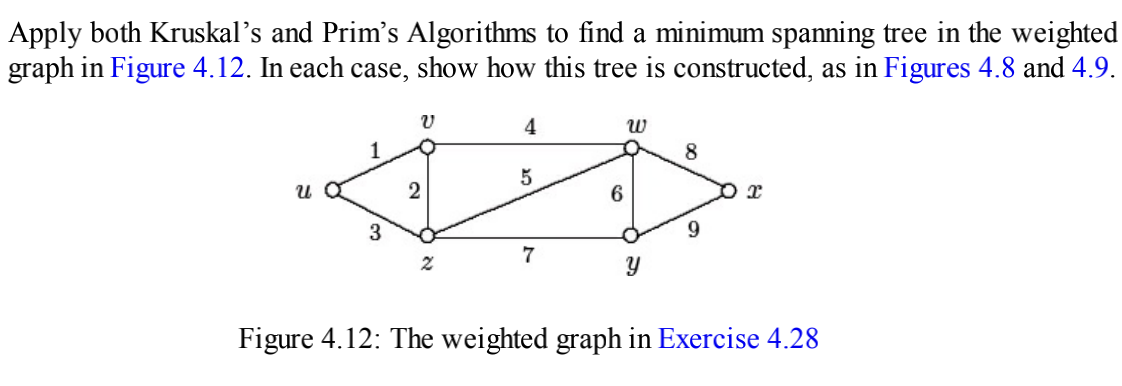
\includegraphics[width = 0.60\linewidth]{figs/b}
  \end{figure}
  
 在图中,若在$c$图中,进队顺序为$x$、$t$,则在拓展时,$x$有可能会拓展到$u$节点,导致在最后的$bfs$树中,存在边$(x,u)$,显然会造成差异。
\end{solution}
%%%%%%%%%%%%%%%

%%%%%%%%%%%%%%%
\begin{problem}
Show that in an undirected graph, classifying an edge $(u,v)$ as a tree edge or a back edge according to whether $(u,v)$ or $(v,u)$ is encountered first during the depth-first search is equivalent to classifying it according to the ordering of the four types in the classification scheme.
\end{problem}

\begin{solution}
若$(u,v)$先被遇到,且顶点$v$是在探寻边$(u,v)$时被首次发现的,则$(u,v)$是一条树边。\\
若$(u,v)$先被遇到,且顶点$v$不是在探寻边$(u,v)$时被首次发现的,则$(u,v)$是一条反向边。\\
反之,若$(v,u)$先被遇到同理。\\
综上,两者等价。
\end{solution}
%%%%%%%%%%%%%%%


%%%%%%%%%%%%%%%
\begin{problem}[TC 22.3-8]
Give a counterexample to the conjecture that if a directed graph G contains a path from u to v, and if u.d < 􏰁v.d in a depth-first search of G, then 􏰁 v is a descendant of u in the depth-first forest produced.
\end{problem}

\begin{solution}
 \begin{figure}[htbp]
    \centering
    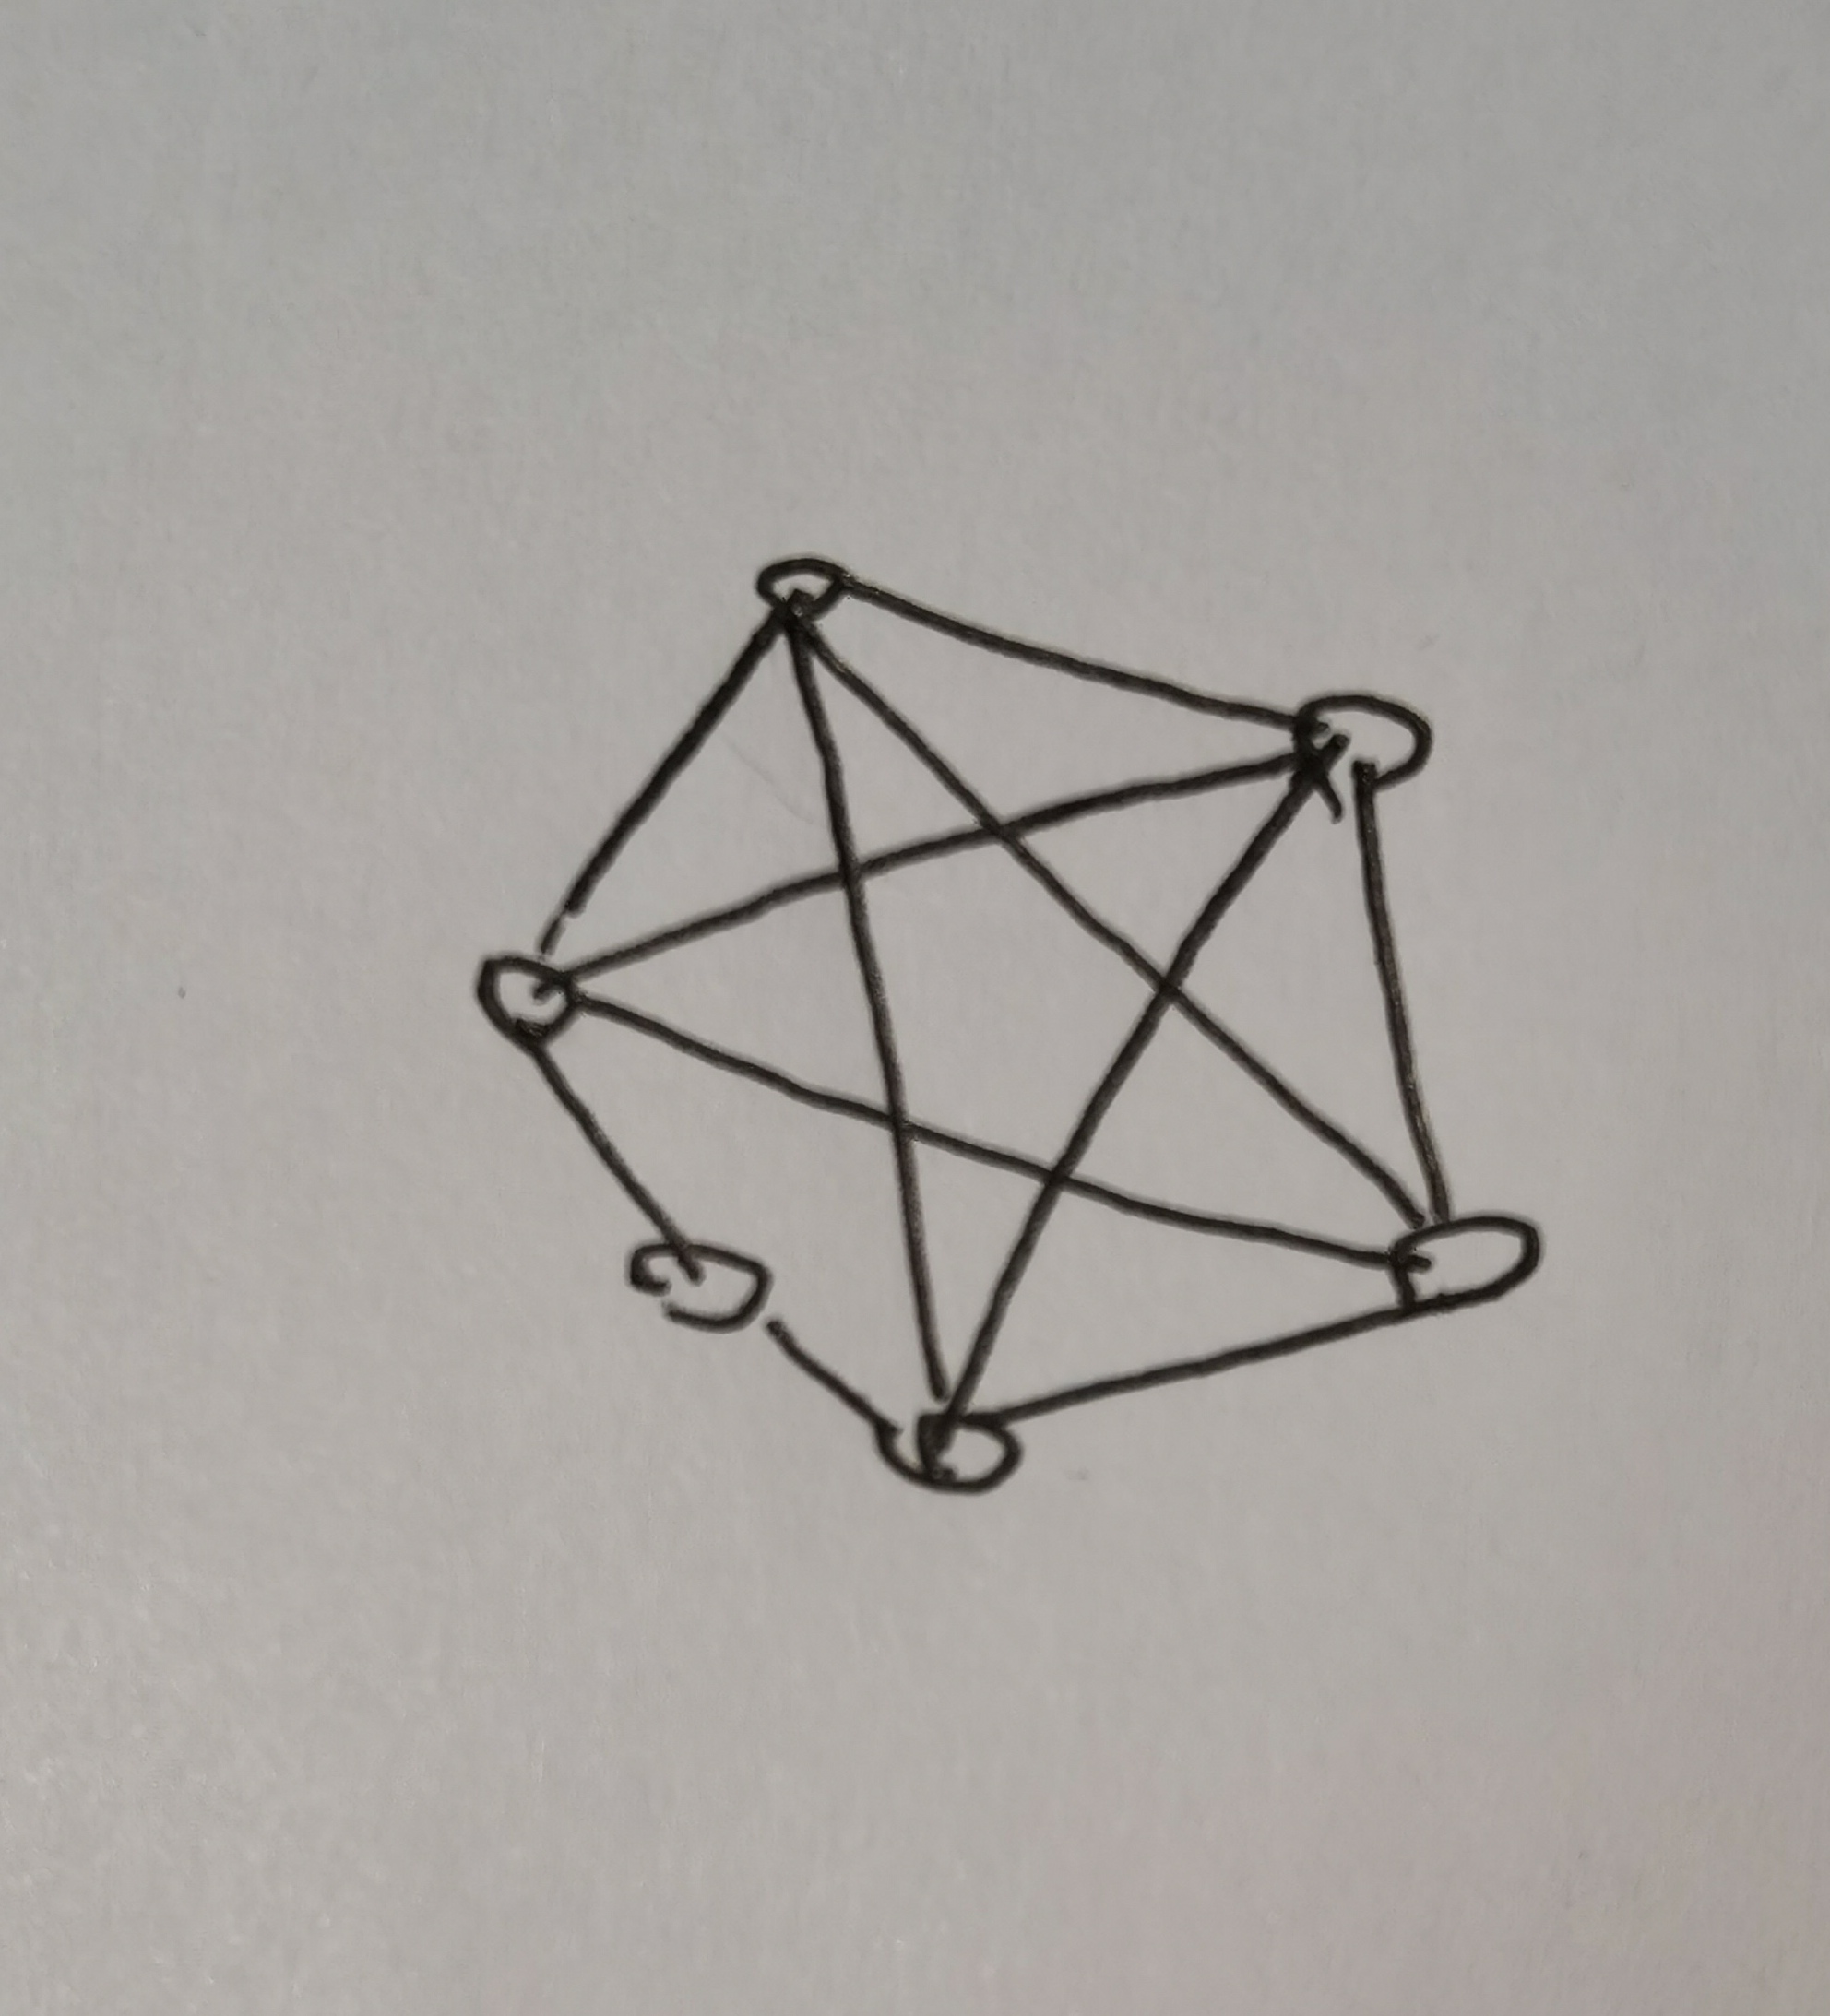
\includegraphics[width = 0.60\linewidth]{figs/c}
  \end{figure}
  如图,若从节点$x$开始遍历,且优先访问节点$u$,则有$d[u]<d[v]$,且在dfs树中,v不为u的后裔。
\end{solution}
%%%%%%%%%%%%%%%
\newpage
%%%%%%%%%%%%%%%
\begin{problem}[TC 22.3-9]
Give a counterexample to the conjecture that if a directed graph $G$ contains a path from $u$ to $v$􏰁, then any depth-first search must result in 􏰁$v.d < u.f$.
\end{problem}

\begin{solution}
 \begin{figure}[htbp]
    \centering
    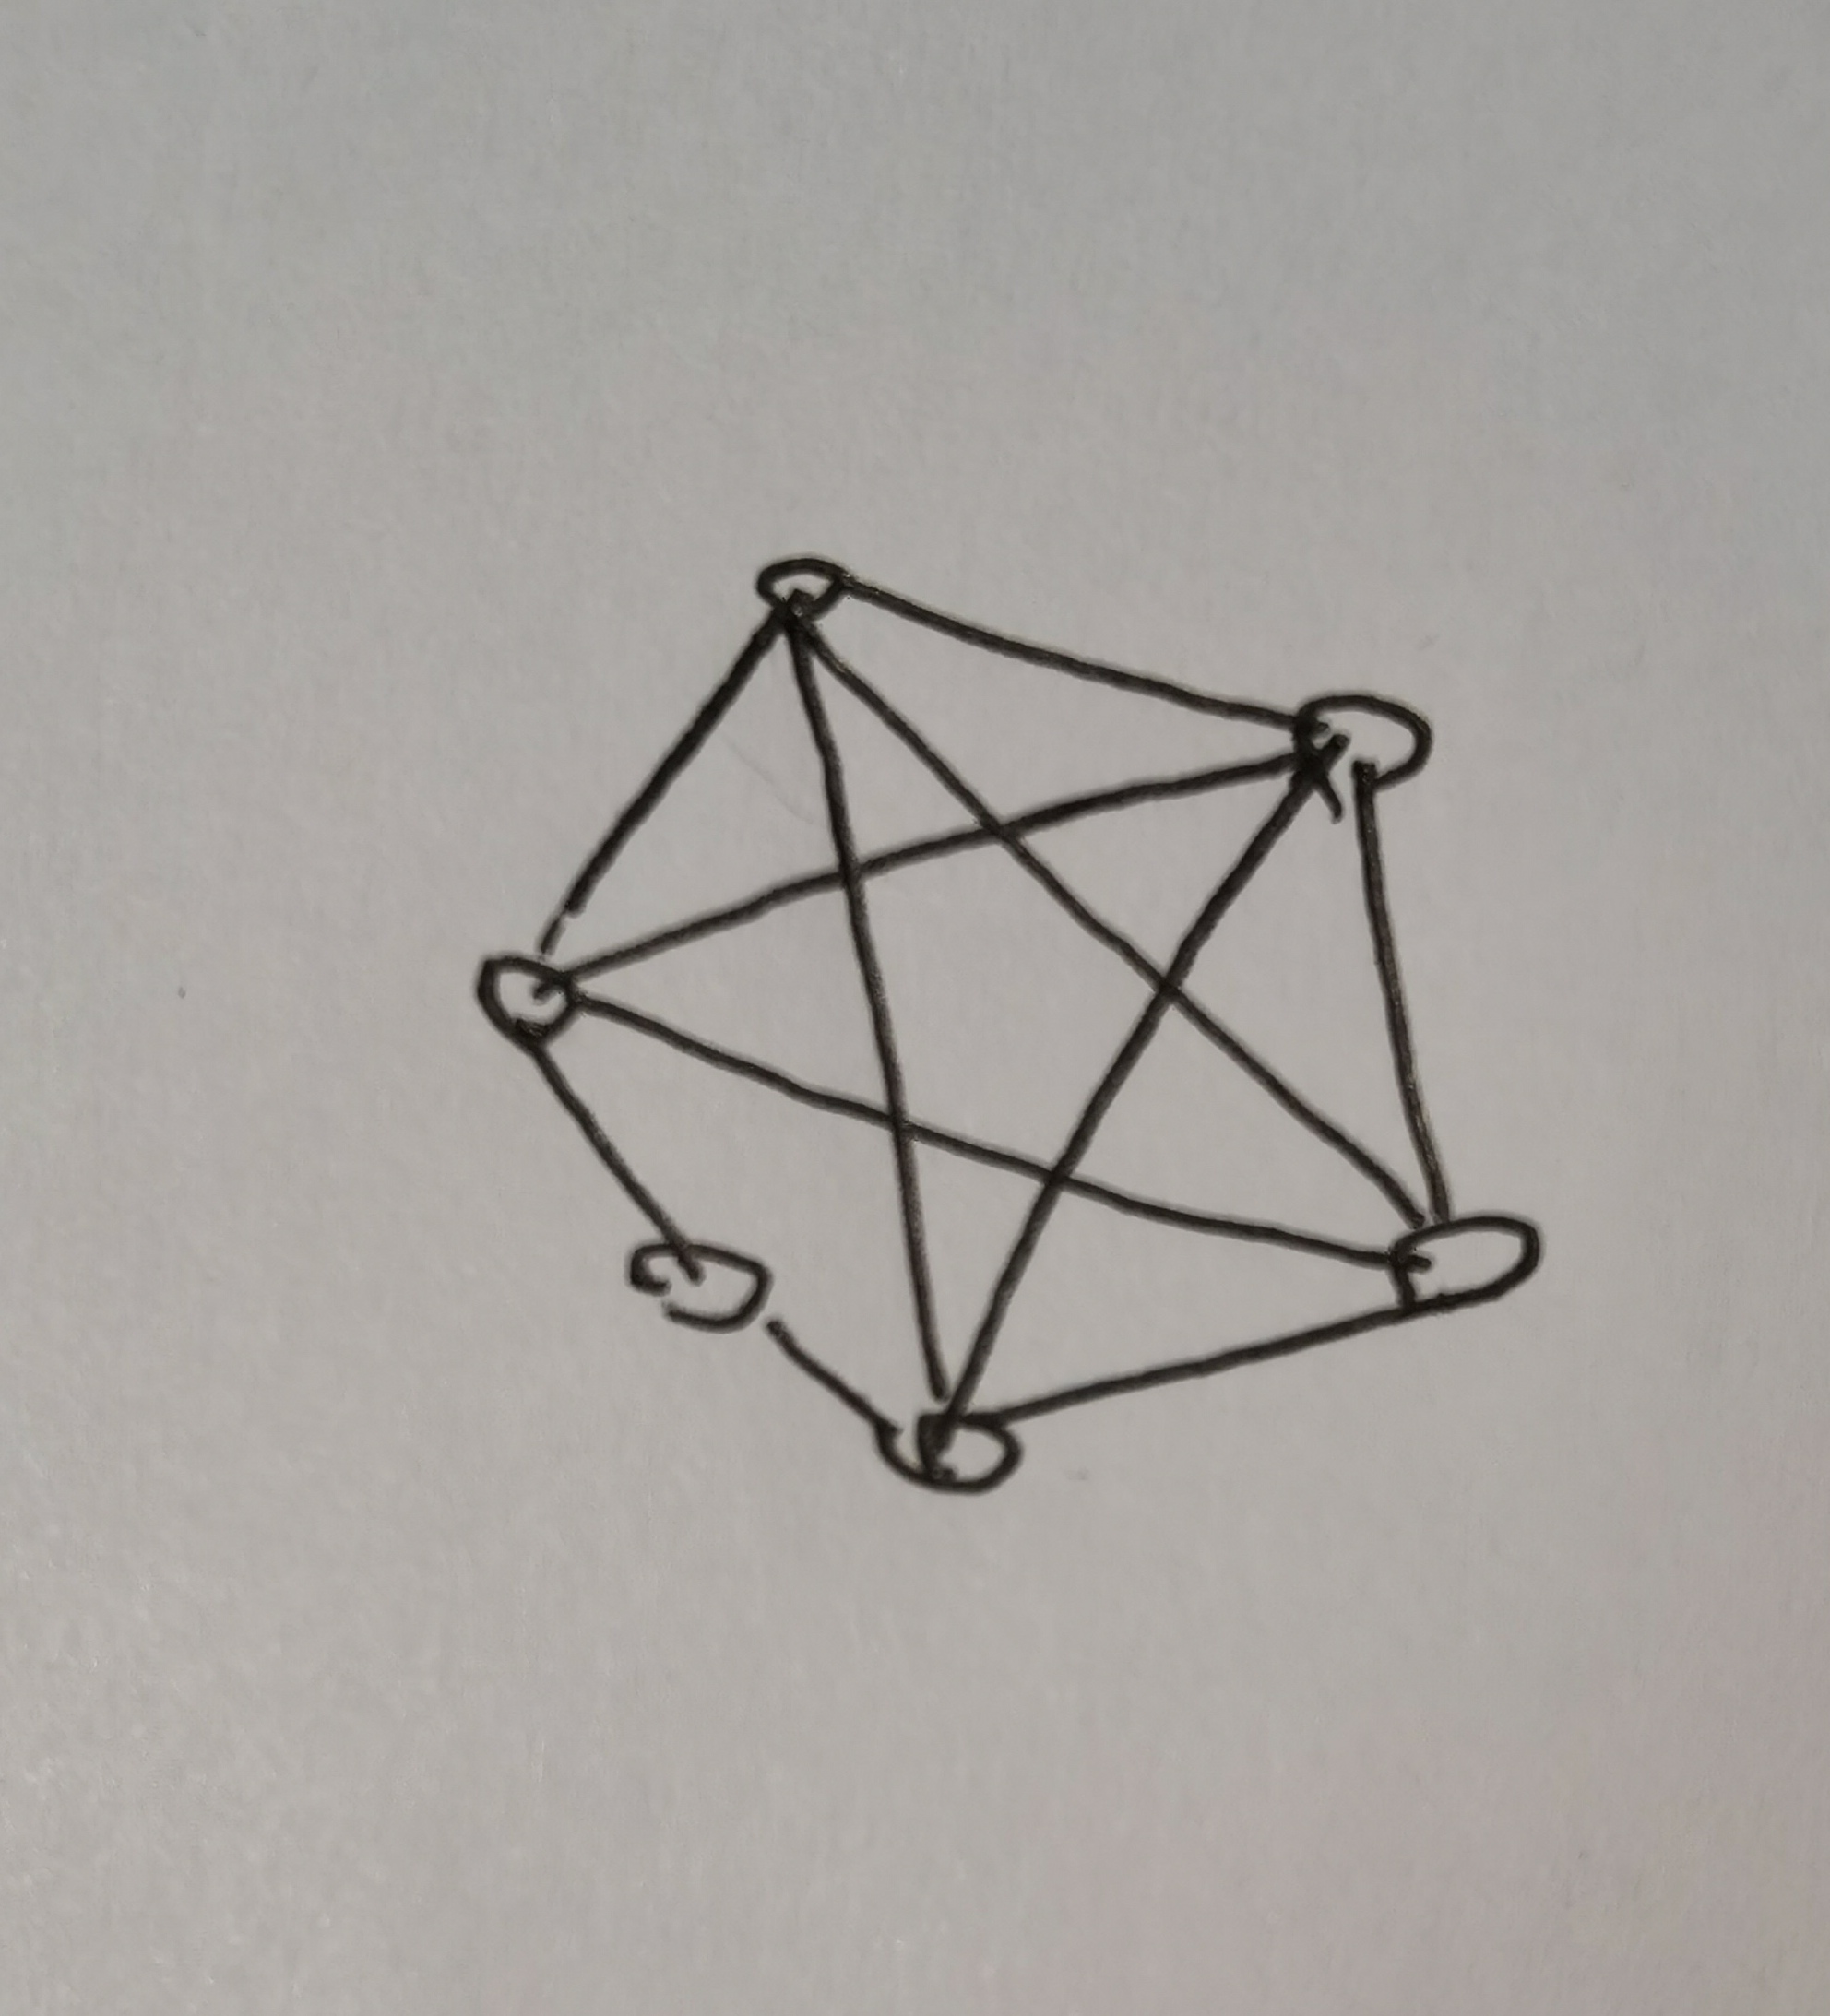
\includegraphics[width = 0.60\linewidth]{figs/c}
  \end{figure}
  如图,存在一条$u$到$v$的路径,若从节点$x$开始遍历,且优先访问节点$u$,则有$d[v]>f[u]$。
\end{solution}
%%%%%%%%%%%%%%%

%%%%%%%%%%%%%%%
\begin{problem}[TC 22.3-12]
Show that we can use a depth-first search of an undirected graph G to identify the connected components of G, and that the depth-first forest contains as many trees as G has connected components. More precisely, show how to modify depth-first search so that it assigns to each vertex 􏰁 an integer label 􏰁:cc between 1 and k, where k is the number of connected components of G, such that u.cc = 􏰁v.cc if and only if u and v􏰁 are in the same connected component.
\end{problem}

\begin{solution}
(1)\\
在无向图中,从一个点开始dfs,则所能遍历到的所有点,一定在一个连通分量中。而所遍历到的点会形成$dfs$树,两个点在一个连通分量中,当且仅当其在一棵dfs树中。故树的数量,即为连通分量的数量。\\
(2)\\
增加全局变量$T$,初始化为$0$。在进入dfs前的循环中,每有一个没被访问需要dfs的点,则$T=T+1$。在dfs中,所有遍历到的点u,进行$cc[u]=T$的赋值。
\end{solution}
%%%%%%%%%%%%%%%

%%%%%%%%%%%%%%%
\newpage
\begin{problem}[TC 22.4-2]
Give a linear-time algorithm that takes as input a directed acyclic graph G=(V,E) and two vertices s and t, and returns the number of simple paths from s to t in G. For example, the directed acyclic graph of Figure 22.8 contains exactly four simple paths from vertex p to vertex 􏰁: po􏰁, pory􏰁, posry􏰁, and psry􏰁. (Your algorithm needs only to count the simple paths, not list them.)
\end{problem}

\begin{solution}
\noindent
\begin{algorithm}
\caption{count}\label{euclid}
\begin{algorithmic}[1]
\Procedure{count}{s, t, G}
\State list $\gets$ TOPOLOGICAL-SORT(G)
\State f[s] $\gets$ 1
\For{u $\in$ list}\Comment{按顺序访问}
	\For{$v : e(u,v)\in G$}
		\State f[v] $\gets$ f[v] + f[u]
	\EndFor
\EndFor
\Return f[t]
\EndProcedure
\end{algorithmic}
\end{algorithm}
\end{solution}
%%%%%%%%%%%%%%%

%%%%%%%%%%%%%%%
\begin{problem}[TC 22.4-3]
Give an algorithm that determines whether or not a given undirected graph $G=(V,E)$ contains a cycle. Your algorithm should run in O(V) time, independent of |E|.
\end{problem}

\begin{solution}
\begin{algorithm}
\caption{cycle}\label{euclid}
\begin{algorithmic}[1]
\Procedure{cycle}{G}
\If{|G.E|$\geq$ |G.V|}
	\State \Return yes
\EndIf
\For {$v\in G.V$}
	\If {!visited[v]}
		\State p $\gets$ dfs(v)\Comment{返回是否有返祖边}
		\If {p == 1}
			\State \Return yes
		\EndIf
	\EndIf
\EndFor
\State \Return no
\EndProcedure
\end{algorithmic}
\end{algorithm}
\end{solution}
%%%%%%%%%%%%%%%

%%%%%%%%%%%%%%%
\begin{problem}[TC 22.5-5]
Give an $O(V+E)$-time algorithm to compute the component graph of a directed graph $G=(V,E)$. Make sure that there is at most one edge between two vertices in the component graph your algorithm produces.
\end{problem}

\begin{solution}

\noindent
\begin{algorithm}
\caption{scc}\label{euclid}
\begin{algorithmic}[1]
\Procedure{scc}{G}
\For {u $\in$ G.V}
	\For {(u,v) $\in$ G.E}
		\If{u.scc $\neq$ v.scc}
			\If {hashmap.find(u,v)} 
				\State continue
			\EndIf
			\State addedge(u, v)
			\State hashmap.insert((u, v))
		\EndIf
	\EndFor
\EndFor
\EndProcedure
\end{algorithmic}
\end{algorithm}
\end{solution}
%%%%%%%%%%%%%%%


%%%%%%%%%%%%%%%%%%%%
\beginoptional

%%%%%%%%%%%%%%%
\begin{problem}[TC 22.5-7]
\end{problem}

\begin{solution}
\end{solution}
%%%%%%%%%%%%%%%


%%%%%%%%%%%%%%%%%%%%
\beginot
%%%%%%%%%%%%%%%
%%%%%%%%%%%%%%%
\begin{ot}[Tarjan's Algorithms]
	[参考资料:\href{https://ieeexplore.ieee.org/document/4569669}{R. Tarjan, "Depth-first search and linear graph algorithms," 12th Annual Symposium on Switching and Automata Theory (swat 1971), East Lansing, MI, USA, 1971, pp. 114-121, doi: 10.1109/SWAT.1971.10.}]
	
\end{ot}

% \begin{solution}
% \end{solution}
%%%%%%%%%%%%%%%

\begin{ot}[带边标记的DFS算法]
	写出带边标记的DFS算法并证明算法的正确性
\end{ot}

% \begin{solution}
% \end{solution}
%%%%%%%%%%%%%%%




% \vspace{0.50cm}
%%%%%%%%%%%%%%%
% \begin{ot}[]
% 
%   \noindent 参考资料:
%   \begin{itemize}
%     \item 
%   \end{itemize}
% \end{ot}

% \begin{solution}
% \end{solution}
%%%%%%%%%%%%%%%

%%%%%%%%%%%%%%%%%%%%
% 如果没有需要订正的题目,可以把这部分删掉

% \begincorrection
%%%%%%%%%%%%%%%%%%%%

%%%%%%%%%%%%%%%%%%%%
% 如果没有反馈,可以把这部分删掉
\beginfb

% 你可以写
% ~\footnote{优先推荐 \href{problemoverflow.top}{ProblemOverflow}}:
% \begin{itemize}
%   \item 对课程及教师的建议与意见
%   \item 教材中不理解的内容
%   \item 希望深入了解的内容
%   \item $\cdots$
% \end{itemize}
%%%%%%%%%%%%%%%%%%%%
% \bibliography{2-5-solving-recurrence}
% \bibliographystyle{plainnat}
%%%%%%%%%%%%%%%%%%%%
\end{document}